\section{Architettura Back-End} \label{sec:archback}

Coerentemente alla struttura imposta dall'adozione di una Clean Architecture, il back-end dell'applicazione è organizzato tramite delle classi controller, use case, repository e data source.\\
Per collegare l'interfaccia grafica lato front-end con il funzionamento dell'applicativo lato back-end, sono state implementate delle server actions per chiamare i controller relativi all'azione desiderata.\\
I controller eseguono la chiamata allo use case relativo, che costituisce ed implementa la business logic dell'intero sistema.\\
Per accedere alle fonti dei dati, necessari a realizzare le funzionalità definite dai casi d'uso, le classi use cases si relazionano con delle classi repositories, nelle quali è posta la logica di persistenza, che presentano i metodi per lettura, scrittura ed eliminazione dei dati.\\
La singola classe repository si interfaccia alla classe data source ad essa associata, la quale presenta i metodi che intervengono concretamente sulle fonti dei dati per compiere le funzioni richieste sui database.\\
Una volta terminate le operazioni nel data source, il controllo torna alla repository, la quale ritorna i dati recuperati allo use case quando richiesto. Completata la funzionalità definita dal caso d'uso, il flusso di controllo torna al controller che dovrà gestire la risposta verso la server action da cui tutto è iniziato.

\begin{figure}[h!]
    \centering  
    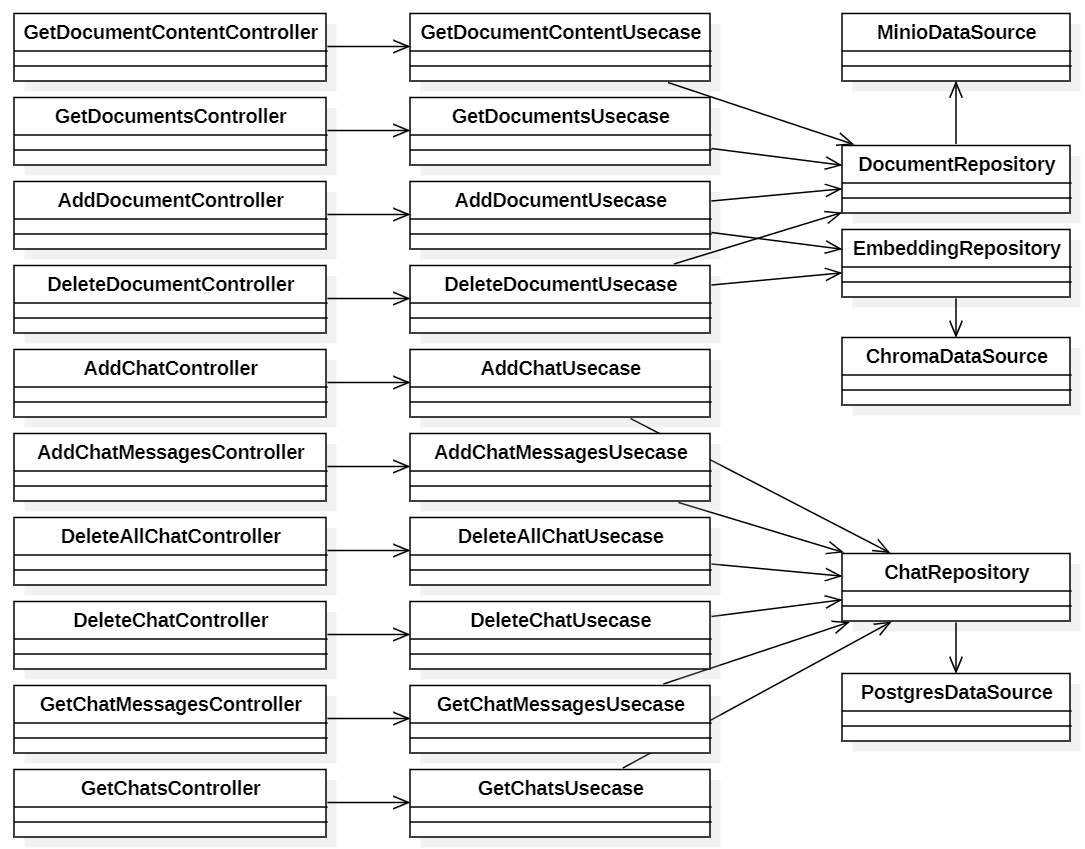
\includegraphics[width=0.7\textwidth]{backendview.png}
    \caption{UML introduttivo delle classi del back-end}
\end{figure}

\newpage
\newpage
